\section{The couplings on the fibre}\label{sec:couplings}

\paragraph{The question.}
Section~\ref{sec:modular} gave the grammar a triplet whose symmetry is a classical modular multiplier. A triplet
becomes physics only when something couples it. We therefore ask what the triplet allows as a coupling, which couplings
the moves allow, and how much of the coupling's shape is fixed before any value is chosen. The answers are exact
statements about one fibre and one modulus $\tau$. They are not statements about the Standard Model, and each carries
the frame in which it holds. The record is cited by its arcs (B1644 to B1666) and by the repository~\cite{OriginAxiomRepo}.

\paragraph{Setting and frame.}
Let $E_\tau$ be the fibre torus with its puncture, carrying the local system of Section~\ref{sec:weave}. By the triplet
postulate (Table~\ref{tab:inputs}) the three holomorphic zero modes, one per parity, are the triplet. Their pairing at
the puncture defines a vector $\rho(\tau)=(\rho_i,\rho_j,\rho_k)$,
\[
  \rho_i=-\frac{\theta_2^2}{2\pi\eta^3},\qquad
  \rho_j=-\frac{\theta_4^2}{2\pi\eta^3},\qquad
  \rho_k=\frac{i\,\theta_3^2}{2\pi\eta^3},
\]
the \emph{theta triplet}, with the arguments $\tau$ and the zero argument understood. (The record writes $R$ for this
vector; we write $\rho$ because $R$ is a move. It is a vector, not the representation $\rho$ of Section~\ref{sec:modular}.) The Higgs lives in the space $\mathcal M$ of the fibre's quaternion
structure, the traceless complex $2\times2$ matrices, spanned by its three imaginary units, with the quadratic form
$a\cdot a$. Two facts are
used throughout.

\begin{lemma}[Jacobi]\label{lem:jacobi}
$\rho\cdot\rho=0$ for every $\tau$.
\end{lemma}
\begin{proof}
By the entries above, $\rho\cdot\rho=(\theta_2^4+\theta_4^4-\theta_3^4)/(2\pi\eta^3)^2$, which
vanishes by Jacobi's identity $\theta_3^4=\theta_2^4+\theta_4^4$~\cite{WhittakerWatson1927}. The same identity gives
$v\cdot v=0$ for the pairing triplet $v(z)=c_r\theta_r(0)\theta_r(z)/\theta_1(z)$ at every point $z$ of the fibre,
through $\theta_4(z)^2\theta_4^2+\theta_2(z)^2\theta_2^2=\theta_3(z)^2\theta_3^2$.
\end{proof}

\paragraph{What the grammar supplies here.}
The grammar supplies the triplet and its multiplier (Theorem~\ref{thm:theta}). The isotropy of the theta triplet is Jacobi's
identity, a classical fact. The fibre frame and the triplet postulate supply the coupling. The results of this section are
what the fibre frame fixes, given the postulate.

\paragraph{Frame dependence, stated first.}
The results of \S\ref{sec:t4} hold in the \emph{fibre frame}: the Higgs is a section on the fibre itself, the zero modes
are the triplet, and the triplet postulate holds at one $\tau$. They fail, or change meaning, in the two other frames on
record. In the surface frame, a reading made within the program, the null vector is not present. In the $E_8$ frame
studied within the program
the Higgs in $\mathcal M$ is a Standard Model singlet, a flavon, and a physical Yukawa coupling needs two condensates, a
doublet--singlet pairing, or the parent map. B1644's and B1649's verdicts carry this scope (B1648, B1655); the frame
tribunal (B1652, Section~\ref{sec:boundary}) finds no frame shown to meet all of the principle's demands alone. Everything in this
section is therefore a statement about the fibre frame and says so.

\subsection{Isotropy and a null vector of the coupling}\label{sec:t4}

For a direction $a\in\mathcal M$, the Higgs in $\mathcal M$ couples the zero modes at the puncture by the symmetric
$3\times3$ matrix
\[
  Y(a)=a\,\rho^{T}+\rho\,a^{T}-(a\cdot\rho)\,\mathbb 1 .
\]

\begin{theorem}[Isotropy and a null vector of the coupling; T4]\label{thm:isotropy}
Given the triplet postulate at one $\tau$, in the fibre frame, with zero Wilson line, the Higgs at the puncture (the
parent map owed), the record's hand, the lifts' agreement with the ruled moves checked at $\Delta^4$ alone, and $M_{1,2}$
as the weave's surface:
\begin{enumerate}
\item (B1644) $\det Y(a)=(\rho\cdot\rho)(a\cdot a)(\rho\cdot a)=0$ for every direction $a$ and every $\tau$. Indeed
  $Y(a)\rho=0=Y(a)^T\rho$: the coupling has a two-sided null vector, the theta triplet (read through the dictionary, one
  massless generation).
\item (B1645) For real $a$ the two other singular values have ratio $m\in[\tfrac12,1]$, set by one angle: with
  $\kappa=2|a\cdot\rho|^2/(|\rho|^2|a|^2)\in[0,1]$ (for real $a$ and isotropic $\rho$, $|a\cdot\rho|^2\le\tfrac12|\rho|^2|a|^2$),
  $m^2=\xi_-/\xi_+$ where $\xi^2-(4+\kappa)\xi+4=0$. The value is $\tfrac12$ for $a$ in the
  plane of $\rho$ and $1$ for $a$ normal to it. $Y(a)$ has rank one exactly on the isotropic cone $a\cdot a=0$, and near
  the cone $m$ grows as $|a\cdot a|/|a|^2$.
\item (B1646) In the unitary frame $(\rho/|\rho|,\bar\rho/|\rho|,n)$ fixed by $\tau$, $Y(a)$ vanishes on $\rho$ and maps
  $\mathrm{span}(\bar\rho,n)$ to $\mathrm{span}(\rho,n)$ by
  $M_2(a)=\begin{psmallmatrix}2(a\cdot\bar\rho)&|\rho|(a\cdot n)\\|\rho|(a\cdot n)&-(a\cdot\rho)\end{psmallmatrix}$, with
  $\det M_2=-|\rho|^2(a\cdot a)$. The map $a\mapsto M_2(a)$ is a linear bijection onto the complex symmetric $2\times2$
  matrices: the direction \emph{is} the mass matrix of the two massive generations.
\item (B1649) For every Higgs $S\in\mathrm{End}(\C^2)$ at the puncture, $\rho$ is a two-sided null vector of the zero
  modes' residue coupling $Y(S)$, which is linear in $S$ ($S=\mathbb 1$ gives the antisymmetric cross product
  $[\rho]_\times$, and $S\in\mathcal M$ gives the formula above). With both quark sectors on one fibre the left massless
  states coincide, so the mixing matrix is $V=1\oplus U(2)$ and $m_u=m_d=\theta_{12}=\theta_{13}=J=0$ at leading order.
\end{enumerate}
\end{theorem}
\begin{proof}[Proof sketch]
(1) is the determinant of a rank-two perturbation of a scalar, $Y(a)\rho=a(\rho\cdot\rho)+\rho(a\cdot\rho)-(a\cdot\rho)\rho$,
which vanishes by Lemma~\ref{lem:jacobi}; B1644 also checks the symbolic determinant. (2) follows from
$s_1s_2=|\rho|^2|a|^2$ and $s_1^2+s_2^2=2|\rho|^2|a|^2+|a\cdot\rho|^2$ for real $a$. (3) is a direct computation in the
frame. (4) uses linearity in $S$ and Lemma~\ref{lem:jacobi} at the puncture; B1649 evaluates the residues by contour
integrals to $5\cdot10^{-31}$. See B1644, B1645, B1646, B1649.
\end{proof}
\noindent\emph{Scope.} The identities are exact. The bound $m\ge\tfrac12$ is exact for real directions (B1645) and does
not hold for complex ones, where $m$ falls to $0.004$ in B1644's numerics. The quartic-potential statement of B1646, that
minima of a potential symmetric under $SO(3)$ and a phase lie on the cone or on the real locus and never between, is for
that quartic; an octic invariant or the zero modes' one-loop term puts minima between (B1655). The statement about
$V=1\oplus U(2)$ is leading order and fibre-frame only. That the $\tau$ of the fibre is a physical modulus is not claimed.

\begin{proposition}[$\rho$ is the residue of the one nilpotent Higgs; B1650]\label{prop:o6}
On the fibre, let $\hat f_r$ be the function with residue one at the puncture and $\hat f_r^{\,2}=\wp(z)-\wp(z_r)$, with each
unit $\mathsf e_r$ at the half-period $z_r$ where its theta function vanishes ($i\leftrightarrow\tfrac12$,
$j\leftrightarrow\tau/2$, $k\leftrightarrow(1+\tau)/2$). The field $\Phi_\rho=\sum_r\rho_r\hat f_r\,\mathsf e_r\,dz$ has
\[
  \Phi_\rho^2=-\Bigl[(\rho\cdot\rho)\,\wp(z)-\sum_r\rho_r^2\,\wp(z_r)\Bigr]dz^2=0,
\]
the second term vanishing identically in the theta constants. So it is a Higgs field nilpotent at every point, and its
residue is $\rho$. Of the six assignments of the units to the half-periods, this is, up to the Klein group's signs,
the only one with this property at a generic $\tau$.
\end{proposition}
\noindent\emph{Proof of the vanishing.} The residues of Lemma~\ref{lem:jacobi} have $\rho_r^2$ proportional to
$(\theta_2^4,\theta_4^4,-\theta_3^4)$ for $r=i,j,k$. With $e_1=\wp(\tfrac12)$, $e_2=\wp(\tfrac{1+\tau}{2})$, $e_3=\wp(\tfrac\tau2)$,
\[
  \textstyle\sum_r\rho_r^2\wp(z_r)\;\propto\;\theta_2^4e_1+\theta_4^4e_3-\theta_3^4e_2
  =\theta_2^4(e_1-e_2)-\theta_4^4(e_2-e_3)=\pi^2(\theta_2^4\theta_4^4-\theta_4^4\theta_2^4)=0,
\]
using Jacobi's identity to split $\theta_3^4$ and the classical $e_1-e_2=\pi^2\theta_4^4$, $e_2-e_3=\pi^2\theta_2^4$.

\noindent\emph{Status.} Verified in B1650 in independent code: $\wp$ is computed through $-(\log\theta_1)''$, whose additive constant
drops out of $\sum_r\rho_r^2\wp(z_r)$ because $\rho\cdot\rho=0$, and the residual is $2.6\cdot10^{-32}$ to $1.7\cdot10^{-31}$ at four values of $\tau$. The five other pairings of units to
half-periods give $0.46$ to $4.96$, except one that also vanishes at $\tau=i$ where $\theta_2=\theta_4$. The
step that a genuine cusp forces a nilpotent residue ($a\cdot a=0$) rests on the tame Higgs correspondence and was not
re-derived in the record (B1650 section 3)~\cite{Simpson1990}. The proposition does not use it.

\subsection{Which couplings the moves allow}\label{sec:t5}

\begin{theorem}[Covariance; T5]\label{thm:covariance}
In the fibre frame, with covariance under the moves invoked where $\tau$ varies (the surface frame, B1651), the move
$L:\tau\mapsto\tau+1$ acts on the pairing triplet as $\mathrm{Ad}(g_L)^{-1}$ and
$R:\tau\mapsto\tau/(\tau+1)$ as $\mathrm{Ad}(g_R)$, with no Klein element, at the puncture and at every half-period
(in the lifts of Theorem~\ref{thm:triplet} this is the lift twisted by the Klein element $i$ on $L$, which accounts for
the inverse). The
half-periods' triplets $(0,-1,i)$, $(i,0,1)$, $(i,-1,0)$ do not depend on $\tau$. The lifts of the moves act on the Higgs space $\mathcal M$ through the
octahedral group $O$ (order $24$), irreducibly. Hence no constant direction $a\in\mathcal M$ is covariant; modulo the
Klein group the twisted moves share exactly the four real body diagonals, so the only covariant class is the real
democratic one.
\end{theorem}
\begin{proof}[Proof sketch]
The covariance identities hold exactly (to $2\cdot10^{-16}$), and a swapped-matrix control fails. Irreducibility of $O$ on the three-dimensional representation, and the common eigenlines of the twisted lifts, are
finite group theory. See B1651.
\end{proof}
\noindent\emph{Scope.} B1655 scopes the corollary B1651 draws, that the Higgs's locus is not forced to the puncture: it
holds for a \emph{point or density Higgs}, a premise that no cell of the arc tests. A Higgs carrying
a parity, in the triplet, couples at the puncture (B1651's addendum). So in the surface frame the covariant loci for an even single-point
Higgs are the puncture, the half-period orbit, or both; in the fibre frame at one $\tau$ any of them is kept (B1651). The
conclusion for other Higgs types is not made.

\subsection{The field stage}\label{sec:field}

The next five statements are propositions: each is exact in its frame, none is a value, and each is stated with its
inputs. They are the steps between a point coupling and a mass matrix.

\begin{proposition}[The rank of a point coupling; B1653]\label{prop:rank}
At the puncture both components of the zero modes behave like $\zeta^{-1/2}$, with $\zeta$ a local coordinate at the puncture, so the residue of a product is a rank-one
bilinear $v_xv_y^T$ of one doublet. Hence for every flat line and every Higgs the record's coupling has rank at most $2$,
and the massless left state is the left field's alone; the four unit residues form a null quaternion
($r_1^2+r\cdot r=0$, with $r_1$ the identity unit's residue and $r$ the line-twisted triplet of the other three, equal to
$\rho$ at $w=0$; on a flat line $r\cdot r\neq0$ in general), so up and down share the left null vector and $V=1\oplus U(2)$ at a point, for every line.
What lifts the zero must not act as a point: two points, a tilted or anisotropic profile, or a profile about the
puncture. A radially symmetric profile about a regular point acts as the point.
\end{proposition}
\noindent\emph{Scope.} Exact (rank $\le2$ at every line on the record to $7\cdot10^{-41}$; two-point and profile controls lift).

\begin{proposition}[The norm of the boundary class; B1654]\label{prop:norm}
The parity Higgs's only massless mode is the boundary class at the puncture. Its norm needs an end cutoff: for the
Szegő kernels of the even spin structures, $\|S_r\|^2_\epsilon=2\pi\log(1/\epsilon)+c_r(\tau)$, where $\epsilon$ is the
radius of a disc removed at the puncture. The \emph{end radius} $\mathcal E$ enters as $\mathcal E=\log(1/\epsilon)$ (the logarithm of a
regulator), and the regularised norm is $2\pi\mathcal E+c_r$. Under equal canonical amplitudes the cutoff's logarithm
cancels by Lemma~\ref{lem:jacobi}: with $\hat\rho_r=\sqrt{2\pi\mathcal E+c_r}\,\rho_r$,
$\hat\rho\cdot\hat\rho=2\pi\mathcal E(\rho\cdot\rho)+D=D$, where
\[
  D(\tau)=\sum_r c_r(\tau)\rho_r^2=\int_{P}\sum_r\rho_r^2|S_r|^2\,dA
\]
is finite and canonical. The first generation's lift is $D/(2\pi\mathcal E)$. $D$ is zero at $\tau=\omega$ (the order-3 move equalises
the norms), $|D|/|\rho|^2$ is modular invariant, and toward the cusp along $\tau=iy$, $D/(q|\rho|^2)=8\pi^2y+8\pi(1-4\ln2)$ up to a relative correction that is
exponentially small in $y$, with $q=e^{i\pi\tau}$. For $\tau=x+iy$ the leading term is
$e^{-i\pi x/2}\bigl[8\pi^2y+4\pi(1+e^{-2\pi ix})-32\pi\ln2\bigr]$, which is the displayed one at $x=0$; the paper's check
\texttt{checks/cusp\_law.py} confirms it at $x=0,\tfrac3{10},\tfrac12,1$ and $y=4,5$.
Under equal framed data there is no lift.
\end{proposition}
\noindent\emph{Scope.} Exact to $1.2\cdot10^{-10}$ by two routes; the direct $D$ to $1.6\cdot10^{-14}$. B1655 scopes it to its
premises (the canonical end condition among them) and finds the lift sensitive to the channels' amplitudes: at $\tau=i$,
$\mathcal E=40$, a $1\%$ error in one channel's amplitude changes it by a factor $2.2$. Which end condition is physical is open. In the flat metric none fixes $\mathcal E$; the fibre's
hyperbolic metric fixes it at order one (Census law~\ref{cl:cusp}). The lift is diagonal along $\rho$, so the light state's angle goes as $1/\mathcal E$.

\begin{proposition}[The lepton sector's null vector at $\tau=\omega$; B1656]\label{prop:electron}
On the stated inputs, namely the eighteen flat lines $w=p_1\tau-p_2$ of exact order nine at $\tau=\omega$, for which $3w$ is fixed by the order-three move, the hypercharge
dictionary (Table~\ref{tab:inputs}, with $6Y$ the
minimal integral normalisation), and B1654's canonical end condition, the charged leptons' first generation stays exactly
massless for every Higgs and every channel weight, while the quarks are lifted.
\end{proposition}
\noindent\emph{Proof sketch.} A flat hypercharge line twists each sector's residue triplet. At $\omega$ the three
perpendicular channels have equal norms, so $D_{\rm sector}=(c_1-c_\perp)r_1^2$, with one gap $-5.806896$. Since $q_L-q_e=-9=-3q_H$
and these lines have $3w$ fixed by the order-3 move, $9w$ lies in the lattice and $r_1({\rm leptons})=\theta_1(-9w)=0$. The
quarks' $|D|/\|r\|^2$, with $r$ the sector's residue, take $1.0312$, $2.4629$, $2.7416$ in a 3-cycle over the lines' classes. See B1656.\\
\emph{Scope.} Given $\tau=\omega$ and these lines, both stated, and the dictionary. Controls off $\omega$, off the fixed lines,
with other charges, and with $r_1$ alone at equal norms all lift. The identification of the dictionary is an input, not a
result, and the minimal normalisation is a choice.

\begin{proposition}[The symmetric point; B1657]\label{prop:symmetric}
At $\tau=\omega$, in the untwisted frame, the Higgs's symmetric vacua are the axes $\rho,\bar\rho,n$ of B1646's frame.
In $\rho$'s basis the order-3 move is the real signed permutation $P$ ($P^TP=\mathbb 1$, $P^3=-\mathbb 1$) with eigenlines
$\rho$ ($e^{-i\pi/3}$), $\bar\rho$ ($e^{i\pi/3}$) and $n$ ($-1$). A Higgs on $n$ gives masses $(1,1,0)$; on $\rho$ or $\bar\rho$ the
coupling has rank one. Near the isotropic vacua the light masses obey two laws, with $d_x=x\cdot x/|x|^2$: for the conjugate
vacuum ($a\approx\bar\rho$, $v\approx\rho$) the light masses over the heavy are $|d_a|$ and $|d_v|$; for the parallel vacuum
($a\approx\rho$, $v\approx\rho$) they are $|d_a+d_v|/4$ and $|d_ad_v|/4$, a geometric hierarchy. Under B1654's canonical end
condition with the Higgs on the line, one generation stays massless and $\mathcal E\,s_2/s_1\to|D|/(2\pi|\rho|^2)$ or
$|D|/(8\pi|\rho|^2)$; $D(\gamma\tau)(c\tau+d)=-D(\tau)$ for the order-3 move makes $D$ a cone at $\omega$.
\end{proposition}
\noindent\emph{Scope.} Untwisted, one fibre, one $\tau$; no cell is blind (B1657). It is a statement about symmetric points
of this frame; it is not a selection of $\omega$ (Section~\ref{sec:selection}).

\begin{proposition}[The twisted half bound; B1658]\label{prop:twisted}
In the twisted frame of B1656, under equal framed data, one Higgs keeps the sectors' second generations within a factor
$4$, exactly. For a null matter residue $M=pq^T$ and any complex Higgs $S$, $\adj Y(S,M)=\det S\,A$ with $A=\tilde q\tilde p^T=A(M)$ (Theorem~\ref{thm:joint}) and
$\|A\|=2\|M\|^2$, and each sector's spectrum is $(1,t,0)$ with $t+1/t=\|Y\|^2/(2|\det S|\|M\|^2)$. The Gram spectrum of $S\mapsto Y(S,M)$ is
$\{1,2,2,4\}\|M\|^2$, so $\|Y\|^2\in[1,4]\|S\|^2\|M\|^2$. One Higgs shares $\det S$, so the sectors' $t+1/t$ lie within a
factor $4$ of each other.
\end{proposition}
\noindent\emph{Scope.} The bound is exact. Its comparison with the measured running masses~\cite{HuangZhou2021} at $M_Z$
is a scoreboard (the data were seen): the ratio for the up quarks against the leptons needs $15.9$, so one Higgs is
refuted \emph{under equal framed data}. Under the canonical end condition the question is B1660's census
(Section~\ref{sec:boundary}), with the same answer for one Higgs.

\subsection{The joint law}\label{sec:joint}

Proposition~\ref{prop:twisted} is the restriction to the null cone of an exact factorisation. In B1656's twisted frame
the Higgs is $S\in M_2(\C)$ and a sector's matter residue is $M=\begin{psmallmatrix}m_0&m_1\\m_2&m_3\end{psmallmatrix}\in M_2(\C)$.
With $\epsilon=\begin{psmallmatrix}0&1\\-1&0\end{psmallmatrix}$ and the three quaternion units
$(C_1,C_2,C_3)=(\epsilon,\ \mathrm{diag}(i,-i),\ \mathrm{diag}(i,-i)\,\epsilon)$, the coupling is the bilinear $3\times3$ matrix
\[
  Y(S,M)_{ab}=\sum_{m,n}\bigl(C_a^{T}\epsilon\,S\,C_b\bigr)_{mn}M_{mn}.
\]
Call $\det S$ and $\det M$ the \emph{defects} of the Higgs and the matter, and $\tr(\epsilon SM^T)$ their \emph{pairing}.

\begin{theorem}[The joint law; T7]\label{thm:joint}
For every $S,M\in M_2(\C)$,
\[
  \det Y(S,M)=4\det S\,\det M\,\tr(\epsilon SM^{T}),\qquad
  \adj Y(S,M)=\det S\,A(M)+\det M\,P\,A(S),
\]
where $P=\mathrm{diag}(1,-1,-1)$ and $A(M)$ is the quadratic
\[
  A(M)=\begin{pmatrix}
  m_0^2+m_1^2+m_2^2+m_3^2 & 2i(m_0m_2+m_1m_3) & -i(m_0^2+m_1^2-m_2^2-m_3^2)\\
  2i(m_0m_1+m_2m_3) & -4m_1m_2 & 2(m_0m_1-m_2m_3)\\
  -i(m_0^2-m_1^2+m_2^2-m_3^2) & 2(m_0m_2-m_1m_3) & -m_0^2+m_1^2+m_2^2-m_3^2
  \end{pmatrix}.
\]
With $N=M\epsilon$ the coupling is symmetric in the Higgs and the matter, $Y(S,N\epsilon^{-1})=Y(N,S\epsilon^{-1})$,
and $\det Y=-4\det S\det N\,\mathrm{polar}(S,N)$, where $\mathrm{polar}$ is the polar form of $\det$. Consequently:
\begin{enumerate}
\item $m_1=0$ if and only if the Higgs is null ($\det S=0$), the matter is null ($\det M=0$), or the pairing vanishes.
\item The squared masses are the roots of $x^3-e_1x^2+e_2x-e_3$ with $e_1=\|Y\|^2$,
  $e_2=\|\det S\,A(M)+\det M\,PA(S)\|^2$ and $e_3=16|\det S\det M\tr(\epsilon SM^T)|^2$. In the hierarchical limit the middle
  mass reads the sum of the two defects' terms, with interference, and the lightest is their product times the pairing over the
  other two masses; both light masses are first order in the defects.
\item At the coincident point $N=S$ the masses are exactly geometric, $m_1m_3=m_2^2$.
\end{enumerate}
\end{theorem}
\begin{proof}[Proof sketch]
Both laws are polynomial identities in the eight entries of $S$ and $M$. B1659 checks them symbolically (residual $0$)
and, for the sector matter of B1656, at $324$ random draws. The symmetric form and the pairing's polar identity
$\tr(\epsilon SM^T)=-\bigl(\det(S+N)-\det S-\det N\bigr)$ are symbolic too. On the null cone $M=pq^T$ the first term of
$\adj Y$ is B1658's $\det S\,\tilde q\tilde p^T$ with the tilde, not the transpose. Item~1 is the vanishing of $e_3$.
Item~3 is the singular-value identity at $N=S$ (to $4\cdot10^{-14}$). The controls fail as expected: the constant $3$ for
$4$, $A$ for $PA$, and $N\neq S$ each break the corresponding identity. See B1659.
\end{proof}
\noindent\emph{Scope.} Exact over $M_2(\C)\times M_2(\C)$, for every Higgs and every matter, in B1656's twisted frame. It
uses no data. It does not say which Higgs or which matter occurs, nor the size of the first generation against nature, and
it is one $\tau$ and a frozen piece of the weave: the interacting weave is not treated. The relation of this frame to the
untwisted frame of Proposition~\ref{prop:symmetric} is not claimed to be a linear equivalence.

\begin{figure}[t]
\centering
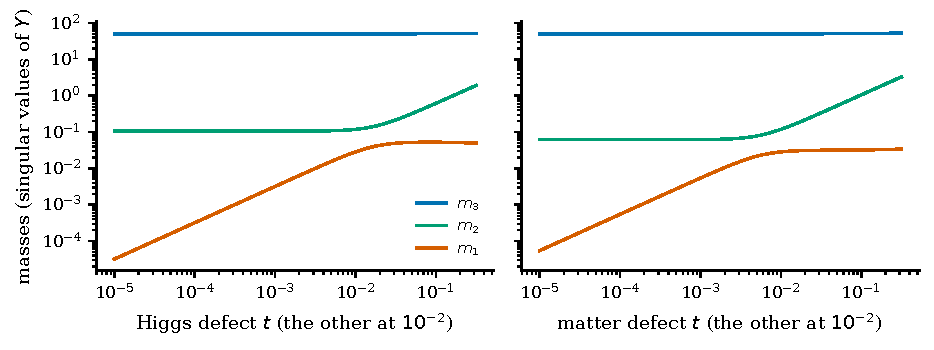
\includegraphics[width=\linewidth]{figures/fig_joint}
\caption{The joint law (Theorem~\ref{thm:joint}): two defects and three masses, an illustrative recomputation from the
theorem's formulas (not an arc's output). In the twisted frame, with a null Higgs and a null matter perturbed by
defects of scale $t$ (left: the Higgs; right: the matter; the other side's defect fixed at $10^{-2}$), the heaviest mass
stays, the middle mass reads the larger defect's term, and the lightest, bilinear in the two defects, falls linearly in
the varied one until it meets the other. Exact identities over $M_2(\C)\times M_2(\C)$ at one $\tau$; no data.}
\label{fig:fig_joint}
\end{figure}

\reading{The coupling's shape is two defects and a pairing. Each defect measures how far a field sits from the null cone;
a null vector is a field, or a pairing, that sits exactly on it. What the grammar fixes is this shape. Where the
fields sit is the choice of a world.}

\subsection{The period phase: the bridge to the motion}\label{sec:phase}

The couplings so far hold at one point of the modular surface. The threads of Section~\ref{sec:weave} are closed paths
through it, and the matter's defect $D$ of Proposition~\ref{prop:norm} is a function along each. How $D$ transforms under
the moves decides how an amplitude built from it can be averaged over a thread.

\begin{lemma}[Automorphy of the defect]\label{lem:automorphy}
The defect $D$ has weight $-1$ and the multiplier $\chi$ of $\eta^6$: for $g=\begin{psmallmatrix}a&b\\c&d\end{psmallmatrix}$
in the modular group, $D(g\tau)=\chi(g)(c\tau+d)^{-1}D(\tau)$, with $\chi(\tau\mapsto\tau+1)=\chi(\tau\mapsto-1/\tau)=i$. Hence $\chi(L)=i$ and
$\chi(R)=-i$ for the two letters of the grammar.
\end{lemma}
\begin{proof}
Write $D=-\theta_3^4h(\lambda)/(4\pi\eta^6)$ with $\lambda=\theta_2^4/\theta_3^4$ and
$h(\lambda)=\lambda\log|\lambda|+(1-\lambda)\log|1-\lambda|$ (the closed form checked in B1657). Under $\tau\mapsto\tau+1$,
$\theta_3\leftrightarrow\theta_4$ and $\theta_2\mapsto e^{i\pi/4}\theta_2$, so $\lambda\mapsto\lambda/(\lambda-1)$ and
$\theta_3^4\mapsto\theta_4^4=\theta_3^4(1-\lambda)$; a short computation gives $h(\lambda/(\lambda-1))=-h(\lambda)/(1-\lambda)$, and
$\eta^6\mapsto i\eta^6$. Hence $D(\tau+1)=iD(\tau)$. Under $\tau\mapsto-1/\tau$, $\theta_3\mapsto\sqrt{-i\tau}\,\theta_3$ and
$\theta_2\leftrightarrow\theta_4$ with the same factor, so $\lambda\mapsto1-\lambda$, $\theta_3^4\mapsto-\tau^2\theta_3^4$,
$h(1-\lambda)=h(\lambda)$, and $\eta^6\mapsto(-i\tau)^3\eta^6=i\tau^3\eta^6$. Hence $D(-1/\tau)=i\,\tau^{-1}D(\tau)$. Both sides of the
law compose by the cocycle rule, and the two maps generate the modular group, so the law holds on the group. The letters
follow from $L:\tau\mapsto\tau+1$ and $R=S_0L^{-1}S_0^{-1}$ (Appendix~\ref{app:hand}).
\end{proof}
\noindent\emph{Remark.} $D$ is real-analytic, not holomorphic, because of $\log|\cdot|$; the law is nonetheless exact. The
record also checks it numerically at $L$, $R$, $S_0$ and $L^{-1}R$, to $10^{-30}$.

\begin{theorem}[The period phase]\label{thm:phase}
Along a thread, let $z(s)$ be the geodesic in the upper half-plane, with $s$ its arclength, and let
$\psi(s)=D(z(s))\,(dz/ds)^{-1/2}$ be the \emph{amplitude}. Then after one period the amplitude returns multiplied by
\[
  \psi(s+\ell)=i^{\,\#L-\#R}\,\psi(s),
\]
the exponent counting the letters of the thread's word $\gamma$. Consequently a coherent average of $\psi$ over a thread survives
only if $\#L\equiv\#R\pmod 4$.
\end{theorem}
\begin{proof}[Proof sketch]
Along a closed geodesic the period is the hyperbolic element $\gamma=\begin{psmallmatrix}a&b\\c&d\end{psmallmatrix}$ of the
thread's word, with $z(s+\ell)=\gamma z(s)$. The derivative $dz/ds$ transforms by $(cz+d)^{-2}$ and $D$ by
$\chi(\gamma)(cz+d)^{-1}$ (Lemma~\ref{lem:automorphy}). Let $r(s)$ be the ratio of the continuation of $(dz/ds)^{-1/2}$
from $s$ to $s+\ell$ to its value at $s$. Then $r^2=(cz+d)^2$. Since $cz+d$ has no zero on $\Hb$ and $r$ is continuous,
$r=\epsilon\,(cz+d)$ with one sign $\epsilon$ for all $s$. As $s\to-\infty$, both $z(s)$ and $z(s+\ell)$ tend to the
repelling fixed point $x$ of $\gamma$ and the two tangent directions agree; for $s$ negative enough the argument of $dz/ds$
varies by less than $\pi$ along $[s,s+\ell]$, so the continued square root takes the principal branch of a ratio that
tends to a positive number (a power of
the ratio of the two heights), while $cz+d\to cx+d$. This is an eigenvalue of $\gamma$, positive because a word in $L$ and
$R$ has positive trace. Hence $\epsilon=+1$, $\psi(s+\ell)=\chi(\gamma)\psi(s)$, and
$\chi(\gamma)=\chi(L)^{\#L}\chi(R)^{\#R}=i^{\#L-\#R}$ because $\chi$ is a character. Census law~\ref{cl:phase} (B1666) checks
this numerically.
\end{proof}
\noindent\emph{Scope.} Exact for every thread, by Lemma~\ref{lem:automorphy} and the argument above. It concerns
$D$ alone, not the physical amplitude, which also needs the Higgs's own transformation (the determinant and the pairing)
that B1656's frame leaves free.

\begin{figure}[t]
\centering
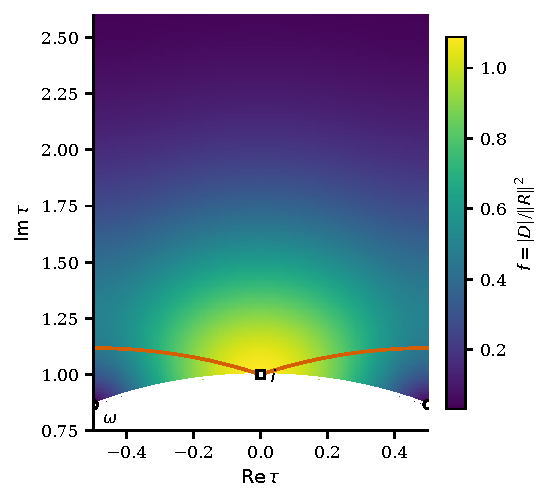
\includegraphics[width=0.55\linewidth]{figures/fig_defect}
\caption{The matter's defect relative to its norm, $f=|D|/\|\rho\|^2$, on the fundamental domain. It is modular-invariant
(Lemma~\ref{lem:automorphy}), vanishes at $\omega$ and toward the cusp, and peaks near $i$. The root $LR$'s closed geodesic,
reduced to the domain, passes through $i$. Computed with the sealed instrument's $f$ (B1663).}\label{fig:defect}
\end{figure}

\begin{censuslaw}[Period phase over the threads; B1666]\label{cl:phase}
On all $30\,674$ threads with trace at most $600$ the least-squares phase over two consecutive periods,
$\sum g(s+\ell)\overline{g(s)}/\sum|g|^2$, equals $i^{\#L-\#R}$ with error at most $1.1\cdot10^{-7}$. The phase is $1$ on
$0.2508$ of the threads, as the four values of the character predict. The ratio includes the square root's branch, so
the census checks numerically the branch sign $+1$ that Theorem~\ref{thm:phase} proves for every thread.
\end{censuslaw}
\noindent\emph{Scope.} A census to trace $600$; no statement for longer threads. It is a sealed test (preregistered, run
once), and the earlier gates that failed at the zeros of $D$ (B1664, B1665) are disclosed in Section~\ref{sec:methods}.

\paragraph{What the bridge shows.}
Two companion readings from the same sealed arc, both scoreboards (the data of B1664 and B1665 were seen, so they are not
blind), are developed in Section~\ref{sec:boundary}. Averaged trace by trace, the threads' average of the defect
$f=|D|/\|\rho\|^2$ approaches the constant mode of the modular surface, $0.31500491$, as the equidistribution of closed
geodesics predicts~\cite{Duke1988,Sarnak1982}; and the amplitude, unlike the size, has no constant wave: its
coherence falls with length. The first is expected, the second is the content. Neither fixes a value of the Standard Model.
